\documentclass[oneside]{article}


\author{Philipp Jetzlaff}
\title{Projektdokumentation}

%packages
\usepackage{fancyhdr}
\usepackage{graphicx}
\usepackage[a4paper, headheight=55pt, bottom=20mm]{geometry}
%Define Header
\fancyhf{}
\fancyhead[R]{
\includegraphics[width=0.11\textwidth]{OktoPOS.png}}
\fancyhead[L]{
  \uppercase{Erweiterung eines Onlineserivce}\\
  \vspace{1pt}
  \small{Anbindung der OktoPOS Software an den internen Übersetzungsdienst}\\ 
  \vspace{4pt}
  \scriptsize{\leftmark}
}
\fancyfoot[L]{Philipp Jetzlaff}
\fancyfoot[R]{\thepage}
\renewcommand{\headrulewidth}{1pt}
\renewcommand{\footrulewidth}{1pt}

%Define Codeblockfont
%Define imagepath
\graphicspath{{src/img/}}
\renewcommand{\listfigurename}{Abbildungsverzeichnis}
\renewcommand{\contentsname}{Inhaltsverzeichnis}
\begin{document}
%Define Header and footer
  \pagestyle{fancy}
  
  %Deckblatt einfügen
  %table of contents
  \pagenumbering{roman}
  \tableofcontents
  \addcontentsline{toc}{section}{\listfigurename}
  \listoffigures
  \addcontentsline{toc}{section}{\listtablename}
  \listoftables
  \newpage
  \section{Verzeichnis der Listings}
  \newpage
  \section{Glossar}
  \newpage
  \pagenumbering{arabic}
  \section{Einleitung}
    Im Rahmen der Abschlussarbeit für den Ausbildungberuft Fachinformatiker für Anwendungsentwicklung 
    wurde diese Projektdokumentation angefertigt. Sie dokumentiert den Ablauf und die Herangehensweise 
    welche zur Lösung, der im Vorfeld von dem zuständigen Ausbilder definierten, Aufgabe beigetragen haben. 
    Der Ausbildungsbetrieb OktoPOS Solutions GmbH ist ein mittelständiges Unternehmen mit Hauptsitz in Hamburg.
  \subsection{Projektbeschreibung}
    Das von der OktoPOS Solutions enwickelte Produkt OkotPOS Cash ist ein, im international Raum, genutztes POS System. 
    Für eine anwenderfreundliche Nutzung ist die gesamte Textausgabe des Front-End in diversen Sprachen konfigurierbar. Zur Realisierung der Textausgabe in 
    den geforderten Sprachen, werden im Quellcode Platzhalter (Tokens) statt konkreter Texte verwendet. 
    FÜr jede Sprache gibt genau eine Property Datei, in der die Texte der jeweiligen Sprache als Key-Value Paar hinterlegt sind.
    Die Erweiterung und Wartbarkeit dieser Property Dateien sind nach aktuellem Stand optimierungsbedürftig. 
    Es gibt keine Garantie dafür, dass jede Datei die selbe Anzahl an Tokens beinhalten bzw. es gibt keinen direkten Überblick über den Übersetzungsstand der Dateien. 
    In den meisten Fällen werden die Übersetzungen von unternehmensfremden Personal angefertigt, die mit der Struktur solcher Dateien nicht vertraut sind und daher mehr Zeit in Anspruch nehmen als notwendig.\\
    Der unternehmensinternen Übsersetzungsdienst TranslationService, bietet neben den grundlegenden Funktionen zum Importieren/Exportieren von Tokens und Übersetzung auch ein benutzerfreundlichen Userinterface.
  \subsection{Projektziel}
    Ziel des Projektes ist es, durch die Anbindung der Kassensoftware an den unternehmensinternen Translationservice,
    den Prozess der Übersetzung von dem Releaseprozess zu entkoppeln und Versionsupdates der Übersetzungen während des Livebetriebes zu ermöglichen.
    Im Rahmen des Projektes soll die Integrität des Kassencodes erhalten bleiben. Deshalb ist es nötig den Updateprozess in eine weitere Anwendung zu überführen. 
    Die Anforderungen der Anwendung sind aus dem Soll-Konzept zu entnehmen.\\
    Der Transaltionservice ist zu so zu erweitern, dass Tokens und Übersetzungen in Abhängigkeit ihrer Version an den Translationservice gesendet bzw. geladen werden können.
    Nach aktuellem Stand, ist der Translationservice nicht in der Lagen die Tokens und Übersetzungen zu Versionieren. Das Anelgen einer neuen Version erfolgt von außen über eine zu schaffende Schnittstelle.
    Im Front-End des Translationservice, soll die Möglichkeit gegeben werden die Tokens und den Stand der Übersetzung nach ihrer Version anzuzeigen.
    Da das Erstellen der Schnittstellen, die Implementierung der neuen Anwendung, das Testen der Komponenten usw. bereits die veranschlagten 70 Stunden benötigt,
    werden das Deployment der Minianwendung sowie die Anpasssung des Deploymentprozesses der Kassesoftware als Fremdleistung an eine andere Abteilung weitergegeben. 
  \subsection{Projektumfeld}
  \subsection{Projektabgrenzung}
  \section{Projektplanung}
  \subsection{Projektphasen}
  \subsection{Vorgehensmodel}
  \subsection{Genutzte Resourcen}
  \section{Analysephase}
  \subsection{Ist-Analyse}
  \begin{figure}[h]
    \centering
    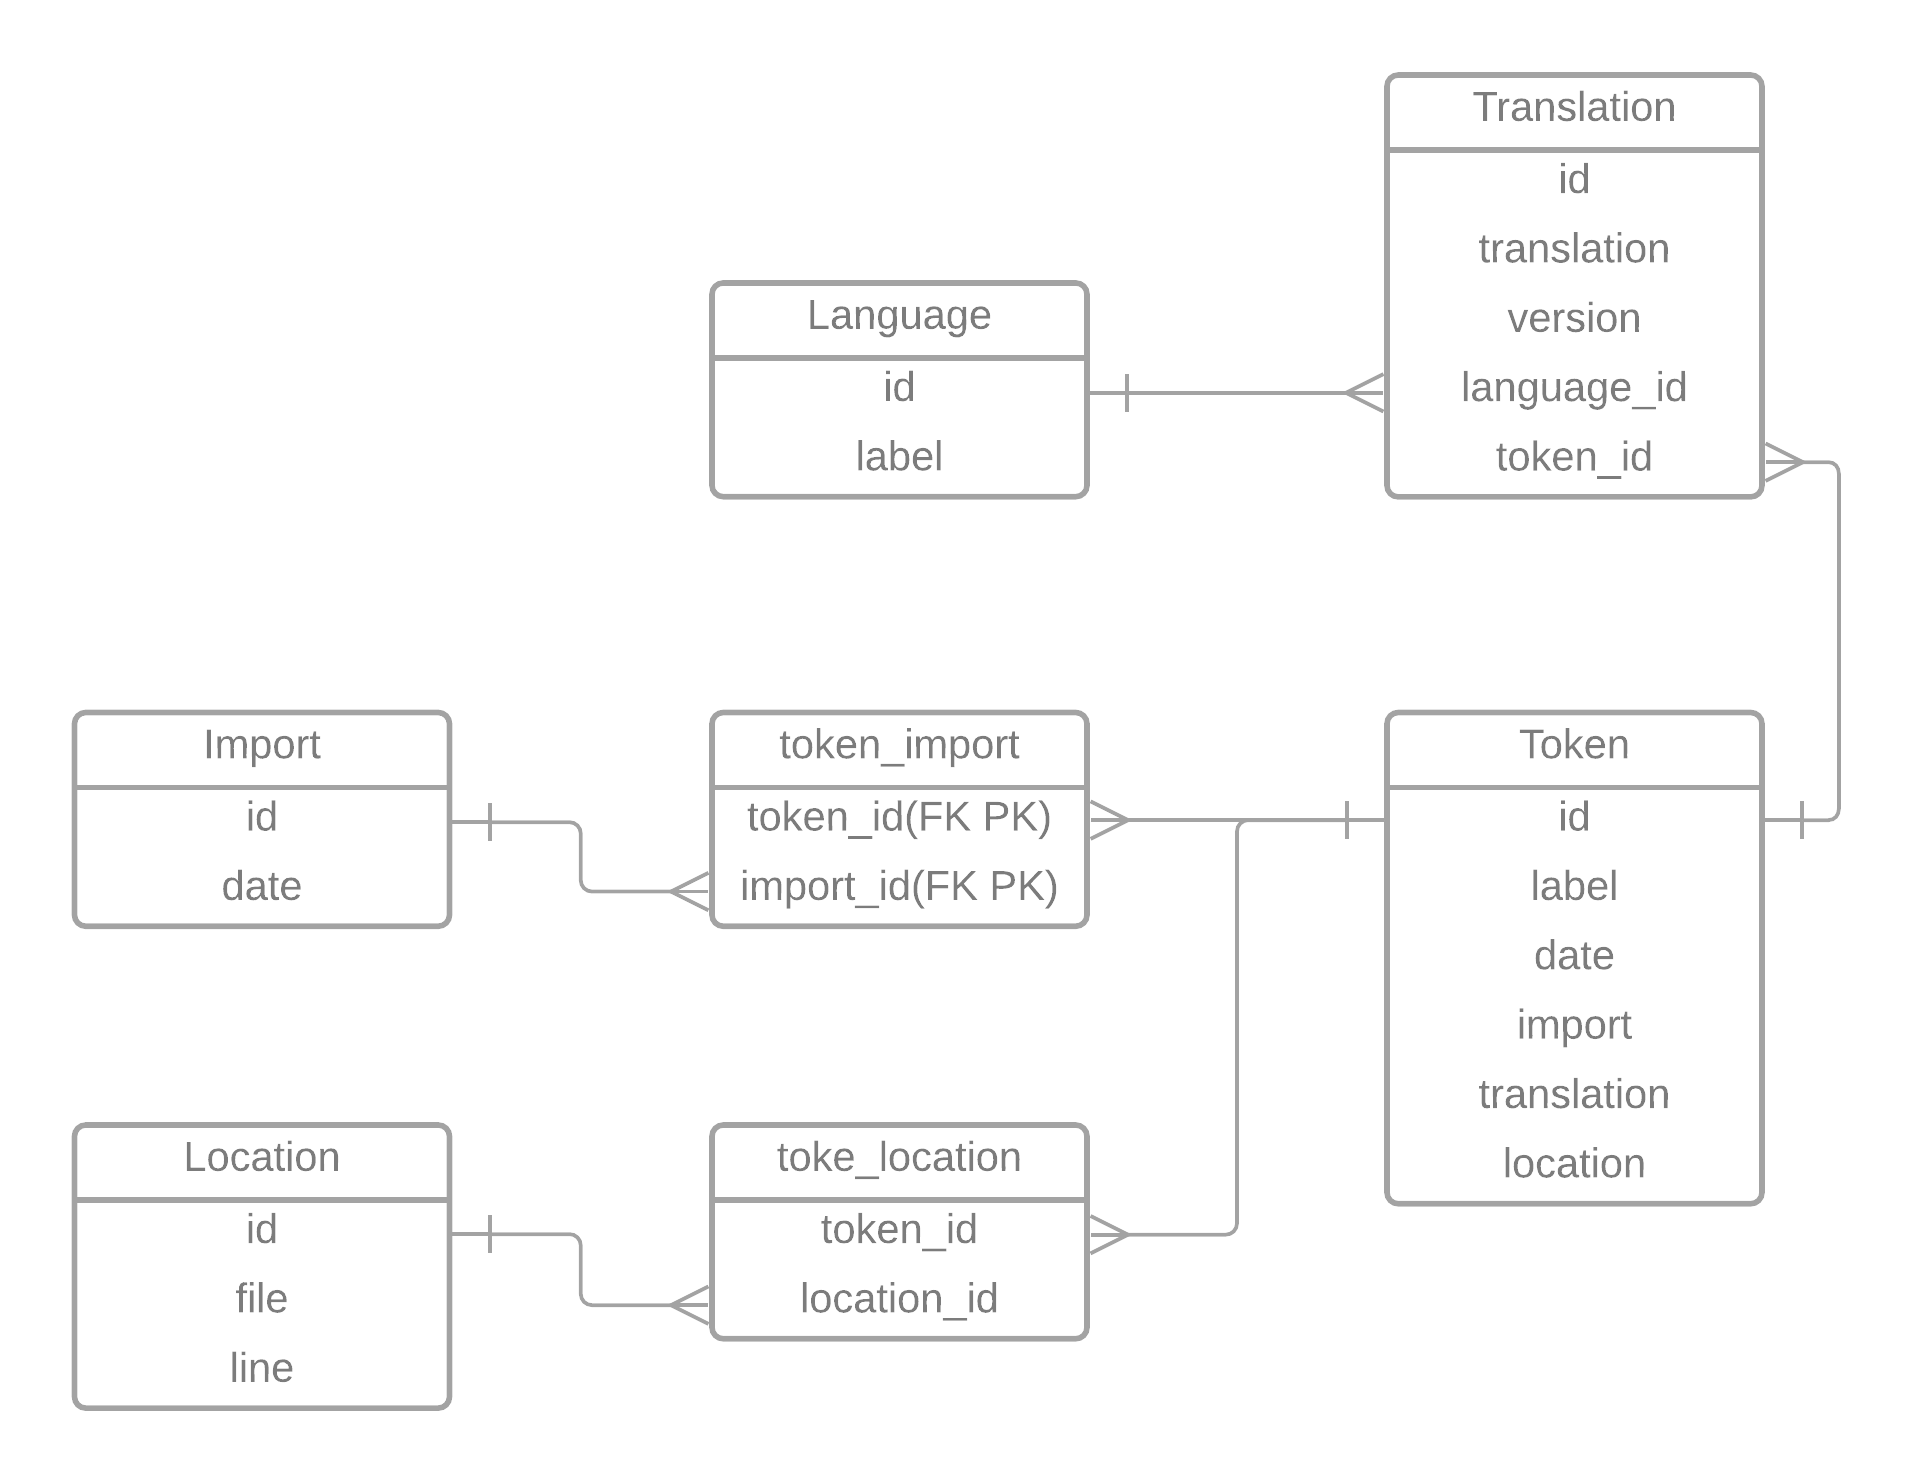
\includegraphics[width=\textwidth]{ERD_TranslationService_IST-Analyse.png}
    \caption{ERD im IST Zustand}
  \end{figure}
  \newpage
  \subsection{Soll-Analyse}
  asd
  \begin{figure}[h]
    \centering
    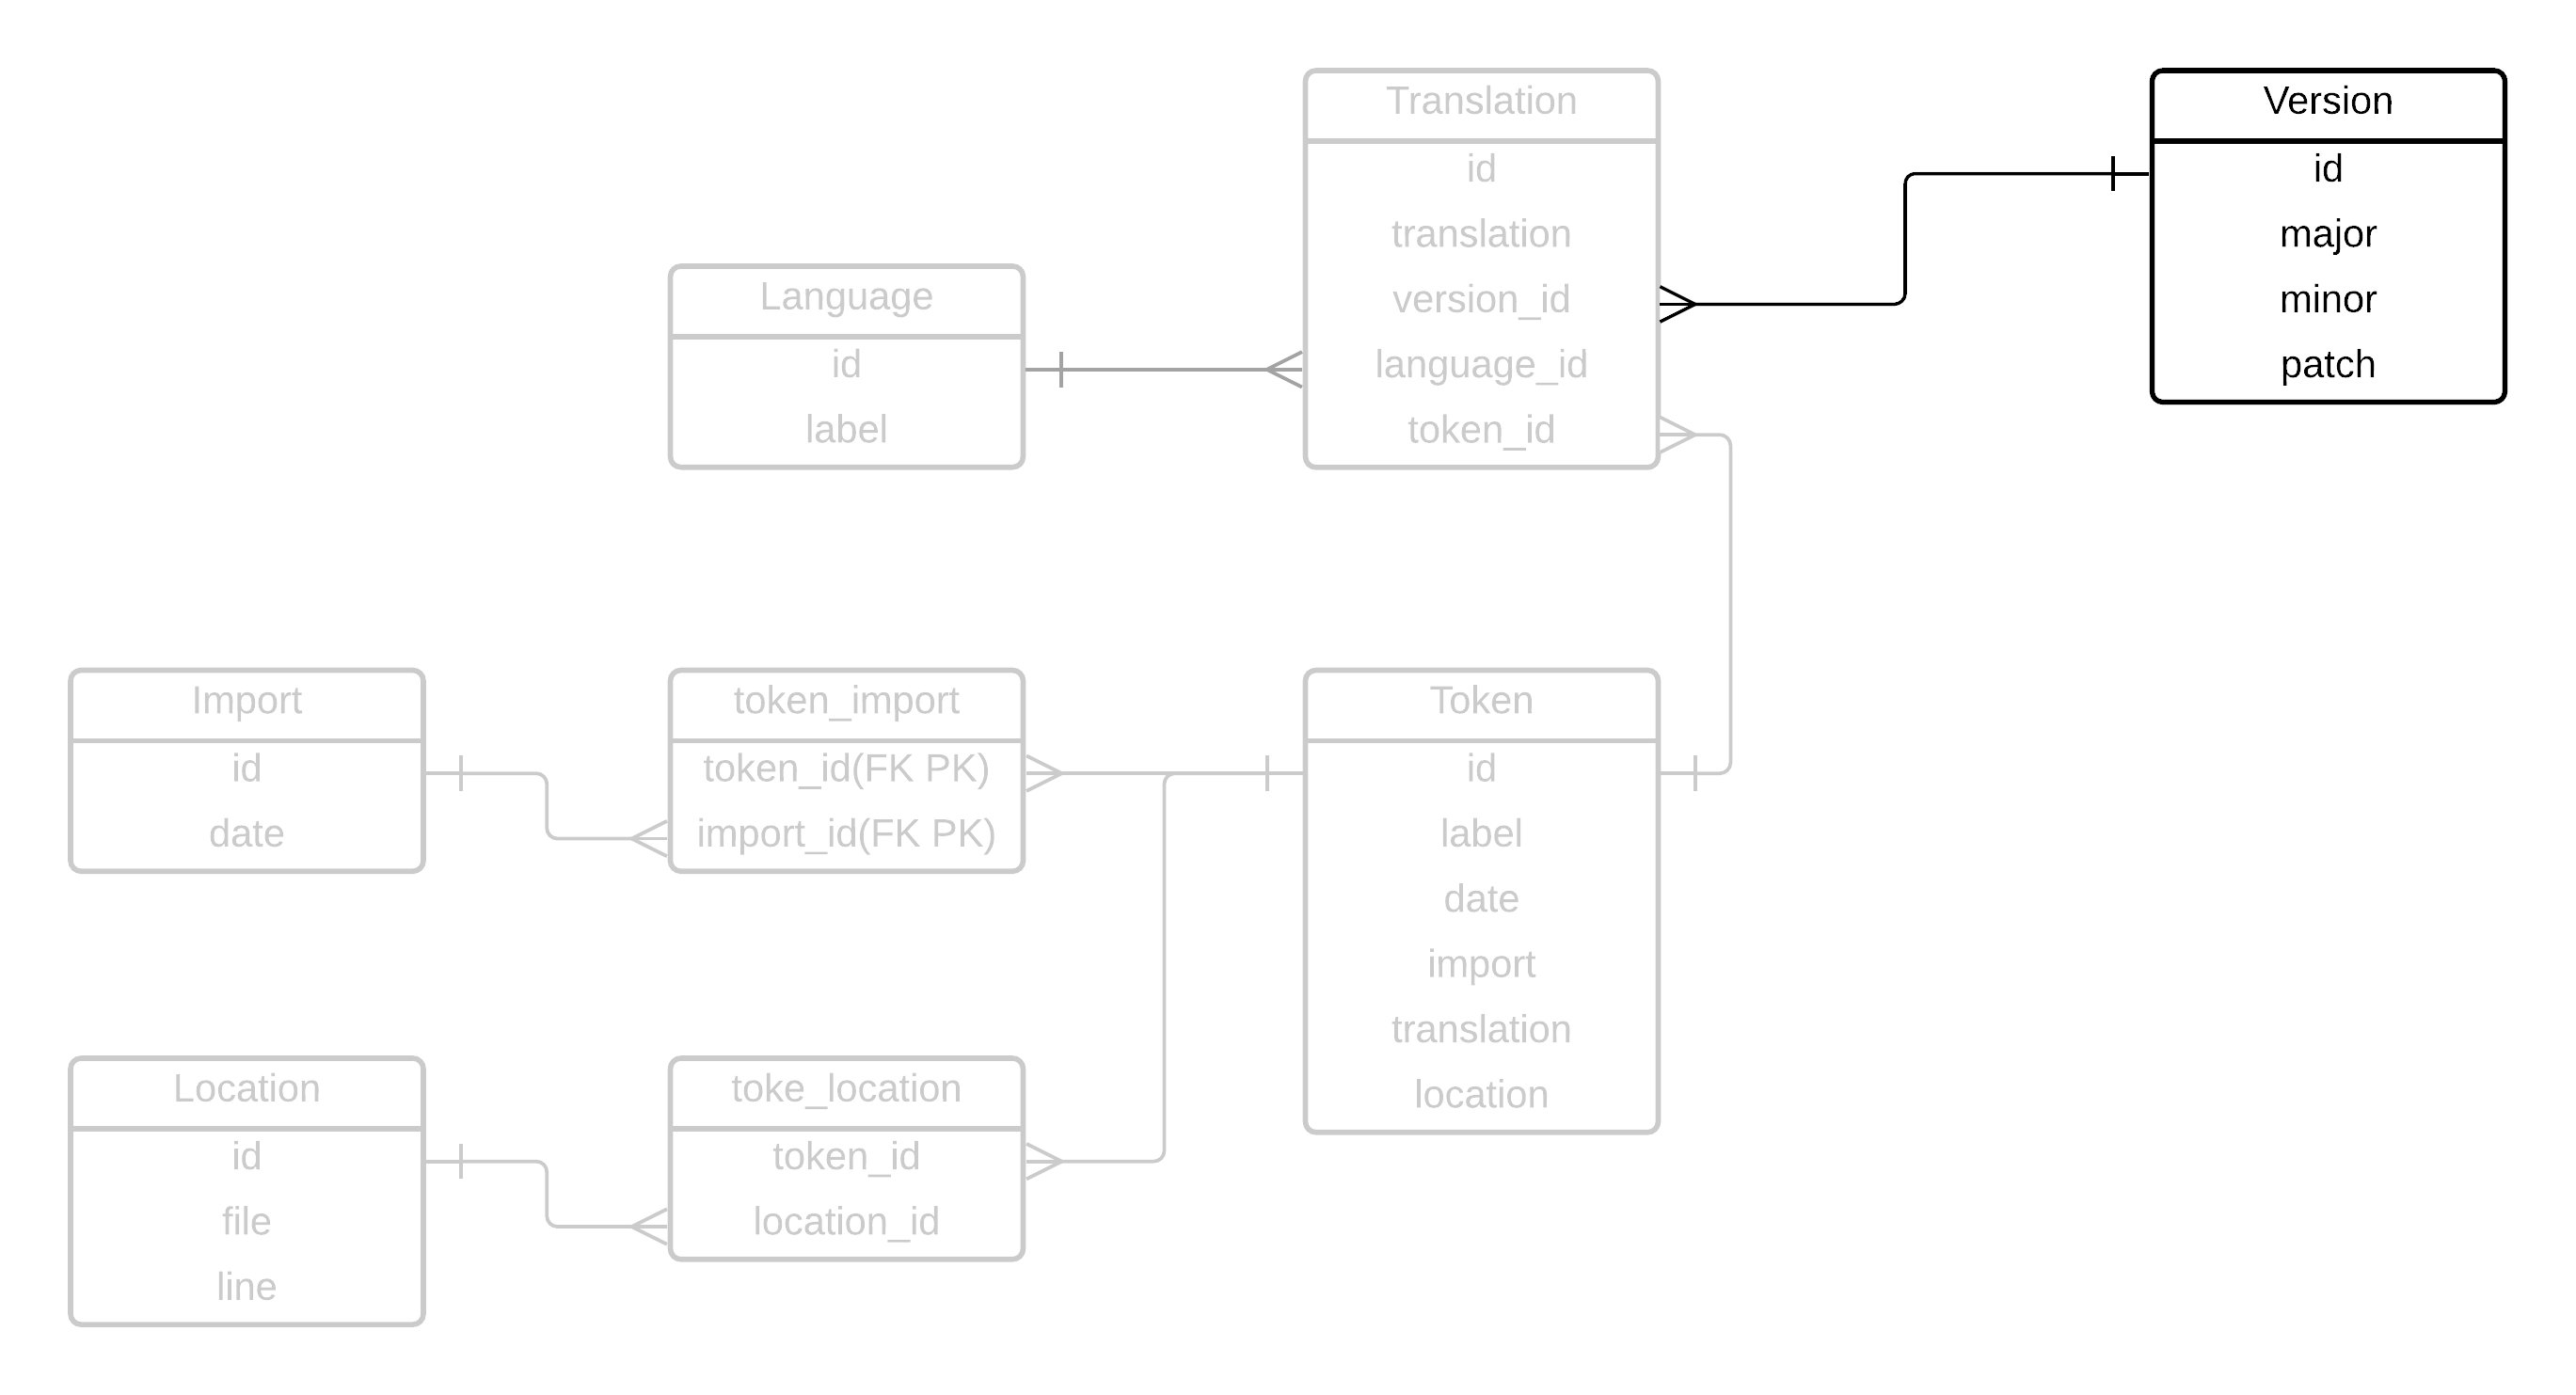
\includegraphics[width=\textwidth]{ERD_TranslationService_SOLL-Analyse.png}
    \caption{ERD im SOLL Zustand}
  \end{figure}  
  \subsection{Wirtschaftsanalyse}
  \subsubsection{Kostenaufstellung}
  \subsubsection{Aromatisierungsdauer}
  \subsection{Anwendungsfälle}
  \subsection{Lastenheft}
  \section{Entwurfsphase}
  \subsection{Userinterface}
  \subsection{Datenmodell}
  \subsection{APIs}
  \subsection{Geschäftslogik}
  \subsection{Testcases}
  \subsection{Pflichtenheft}
  \section{Implementierungsphase}
  \subsection{Translationservice}
  \subsubsection{Erweiterung der bestehenen Datengrundlage}
  \subsubsection{Implemetierung der REST Api}
  \subsection{Translationloader}
  \subsubsection{Geschäftslogik}
  \subsubsection{Userinterface}
  \subsubsection{Batch Script Extension}
  \subsubsection{Webhook}
  \section{Abnahme- und Einführungsphase}
  \subsection{Abnahme durch den Fachbereich}
  \subsection{Deployment}
  \section{Dokumentation}
  \section{Retroanalyse}
  \subsection{IST-SOLL-Vergleich}
  \subsection{Ausblick}
  \setcounter{section}{0}
  \renewcommand{\thesection}{\MakeUppercase{\alph{section}}}
  \section{Anhang}
  \subsection{Schnittstelledokumentation}
  Swagger
\end{document}